\documentclass[11pt,a4paper,twoside]{article}
\usepackage[utf8]{inputenc}
\usepackage{amsmath}
\usepackage{amsfonts}
\usepackage{amssymb}
\usepackage{graphicx}
\usepackage{physics}
\usepackage{mathtools}
\usepackage{bm}
\author{François Coppens}
\title{Notes}
\renewcommand{\vec}[1]{\bm{\mathrm{#1}}}
\newcommand{\unit}[1]{\,\mathrm{#1}}
\begin{document}

	Superfluids are liquids and gasses with remarkable properties. In particular, superfluid helium can flow through a capillary without friction[\emph{ref}] due to its extremely low viscosity[https://doi.org/10.1016/j.crhy.2017.10.016]($\approx\!1500$ times lower than normal liquid helium), or creep up the wallof a container, seemingly defying the force of gravity (``Rollin creeping'')[\emph{ref}]. Its thermal conductivity is about $3\times10^6$ times higher[\emph{ref}] than that of typical liquids and about 200 times higher[\emph{ref}] than that of copper at room temperature[https://doi.org/10.1016/S0031-8914(36)80312-7,https://doi.org/10.1038/140062a0]. It therefore earned the title of ``best heat conducting substance we know'' by Willian and his daughter Anna Keesom and dubbed `\emph{supra-heat-conducting}'[\emph{ref}]. Later it was understood why[\emph{ref}] and it turns out that heat doesn't diffuse through the medium as in normal liquids, but rather it travels through the medium in waves (second sound). This makes it an ideal coolant e.g. to stabilise the superconducting magnets in CERN's Large Hadron Collider. Helium is also the only known substance that stays liquid at zero temperature and low pressures and both it's angular momentum and vorticity are quantised, making it the first observed macroscopic quantum substance. Helium-4 becomes superfluid below the$\lambda$-point, named so by William H. Keesom in 1936 who measured a singularity in the specific heat at $T_\lambda=2.2\unit{K}$.[https://doi.org/10.1016/j.crhy.2017.10.016]\\
	
	\begin{figure}
		\begin{center}
			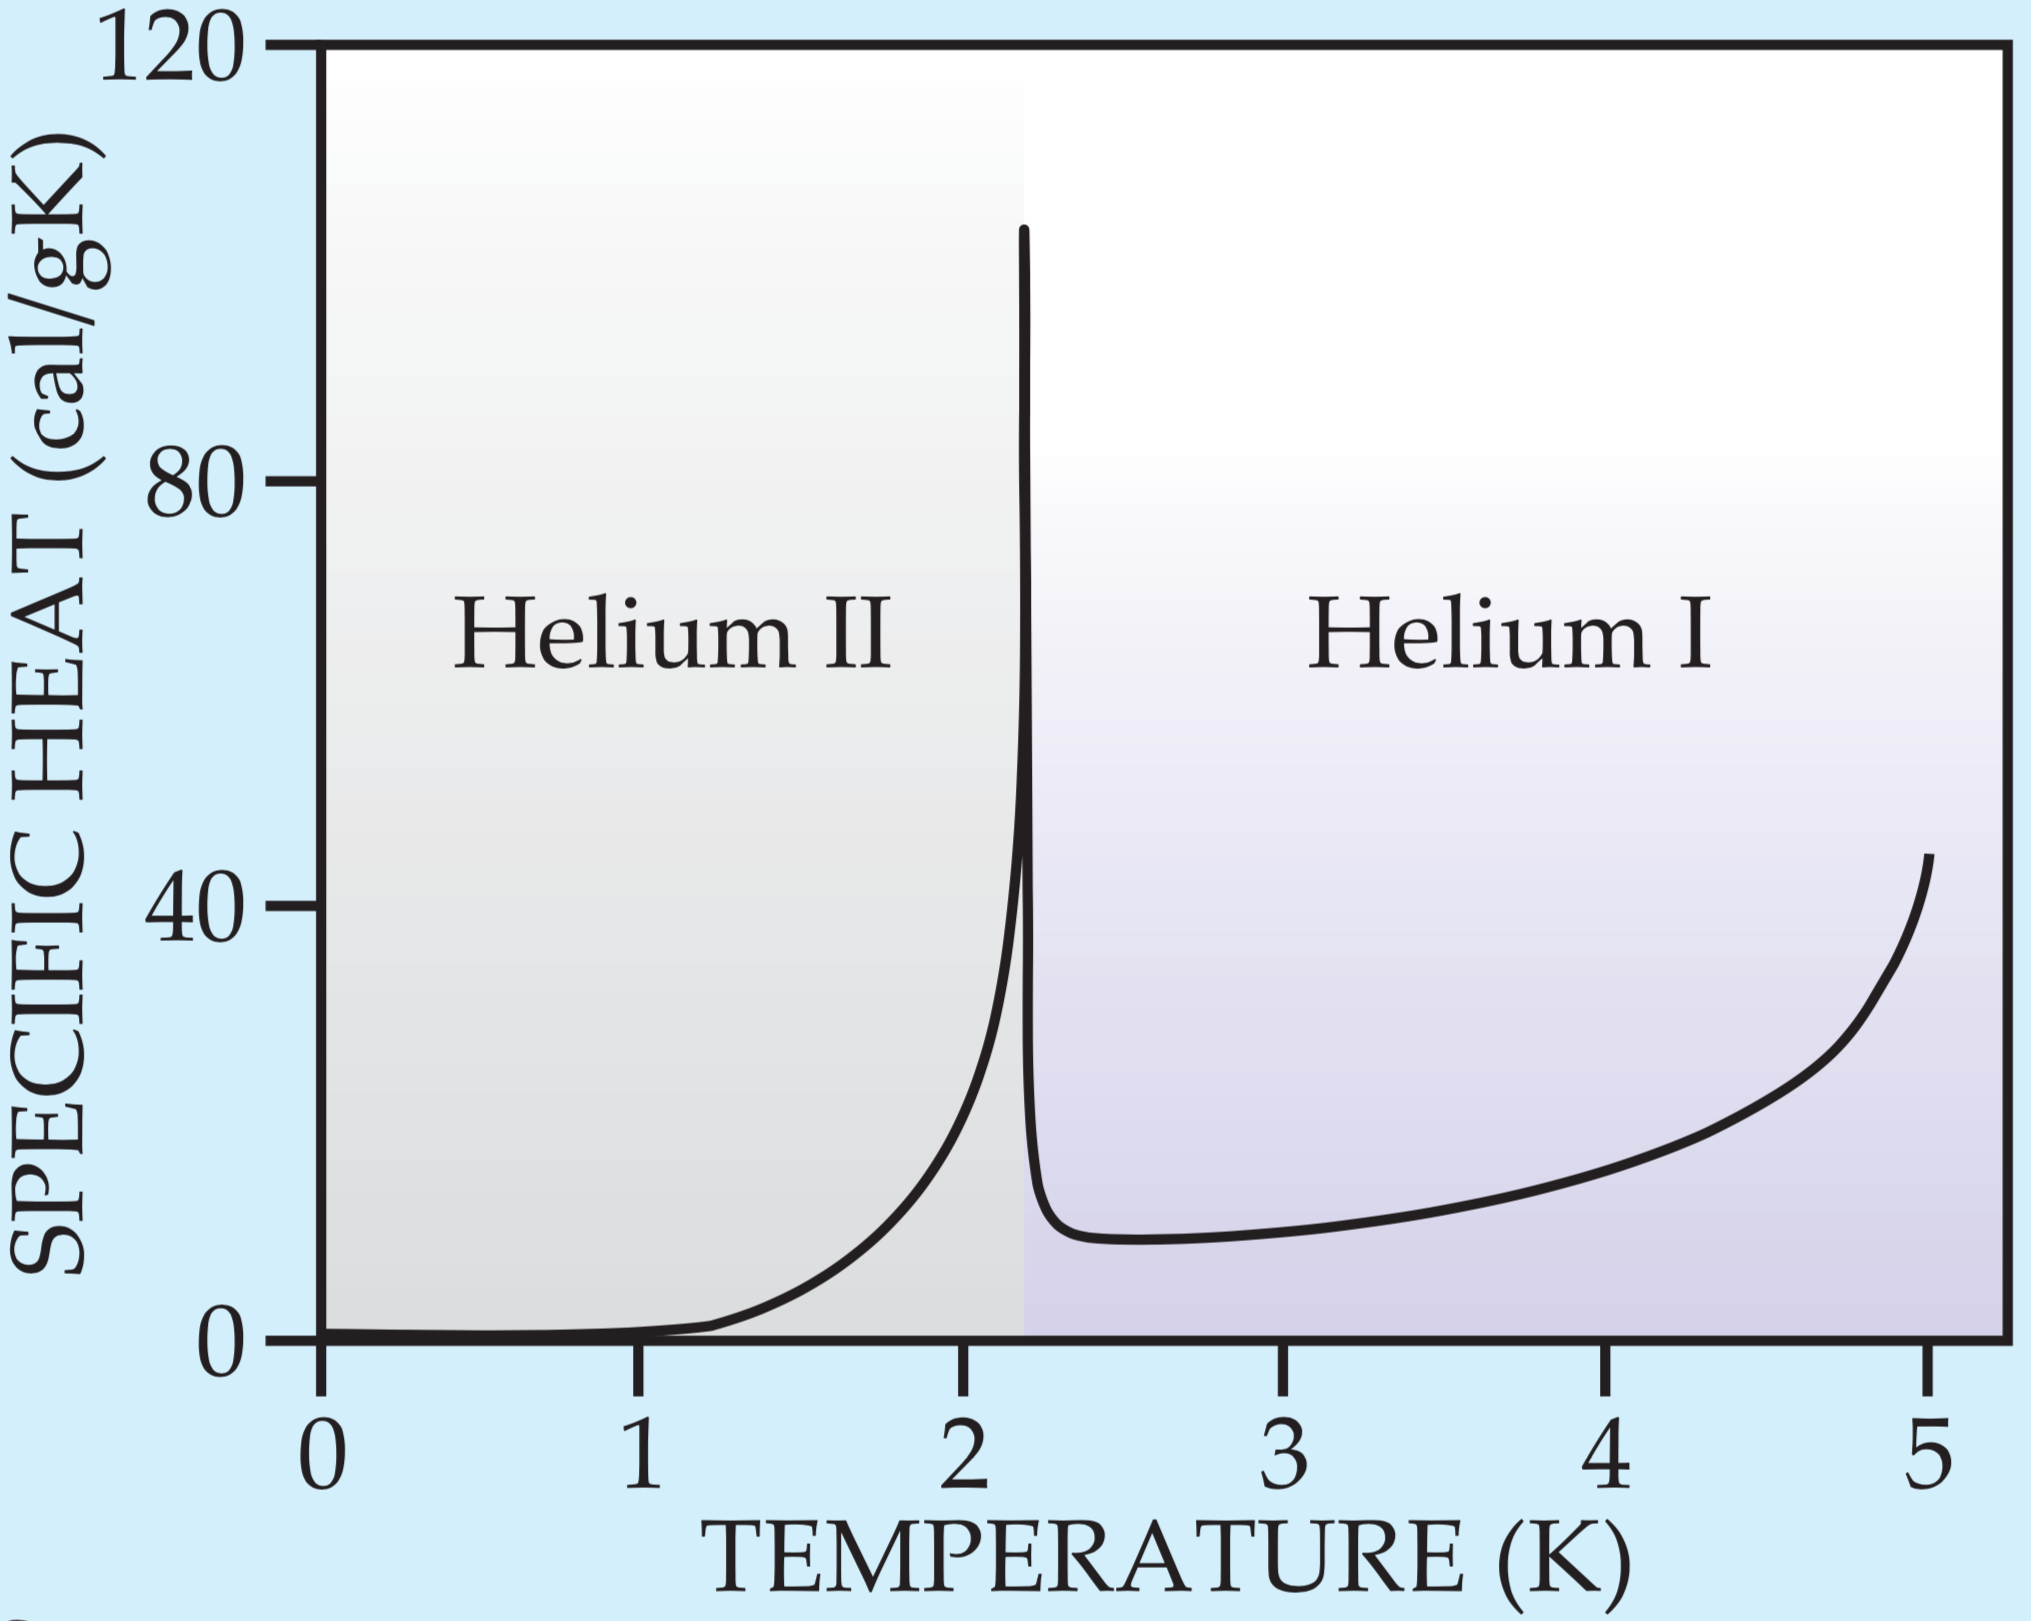
\includegraphics[width=0.45\textwidth]{specific-heat}
		\end{center}
		\caption{The specific heat of $^4$He as a function of the temperature.}
		\label{fig:specific-heat}
	\end{figure}	
	
	Helium was the last gas to be liquefied and was done so by Kamerlingh Onnes in 1908[\emph{ref}]. In 1932 John McLennan saw[\emph{ref}] that liquid helium stopped boiling below $\approx2.2\unit{K}$ and later that year Willem Keesom and his daughter Anna observed[\emph{ref}], while measuring  the temperature dependence of the specific heat, a singularity around the same temperature. They called it the ``$\lambda$-temperature'',  $T_\lambda$, because of the shape of the temperature dependence of the specific heat resembling the Greek letter $\lambda$ (see Figure \ref{fig:specific-heat}). A few years later in 1935 Burton measured a sharp decrease in the viscosity of liquid helium below $T_\lambda$. Around the same time Fritz London was already thinking about macroscopic wave functions and why helium does not freeze at $T=0\unit{K}$ under atmospheric pressure. He concluded that it was caused by the zero point motion of the helium atoms and of their associated kinetic energy that was comparable to their Van der Waals energy, effectively preventing liquid helium to solidify. The year after, in 1936, Willem and Anna Keesom measured an abnormally high heat conductance below $T_\lambda$. This was confirmed roughly one year later by J.F. Allen \emph{et al.} and it was understood that the high thermal conductance was the reason for the helium to stop boiling whenever the temperature drops below $T_\lambda$. It was in 1937 when Kapitza tried to determine the viscosity of the laminar flow that he measured a viscosity that was about $10^4$ times smaller than that of hydrogen gas. It was then that Kaptiza who, by analogy with superconductors, first coined the word ``superfluid'' to describe the special state that helium enters below the $\lambda$-point where it can flow, seemingly without friction. Allen and Misner realised that superfluid helium is not just a liquid with a very low viscosity, but that its hydrodynamics was completely different from that of ordinary liquids and therefore required a completely new interpretation. The start of this new interpretation was made by London in 1938 when he made a connection between the behaviour of superfluid helium to that of an ideal Bose-Einstein gas. Both his calculated value for $T_c=3.09\unit{K}$ and the behaviour of the temperature dependence of the heat capacity for the ideal Bose-gas were very similar to the measured ones for liquid helium below $T_\lambda$. He wrote to Nature that ``it was difficult not to imagine a connection with Bose-Einstein condensation''. Laszlo Tisza expanded upon London's ideas and considered a Helium II system of total $N$ atoms to consist of two parts; a macroscopic ``condensed'' part $n_0$, the superfluid component, in the ground state, and the remaining part $n=N-n_0$, the normal component, where the helium atoms are distributed over the excited states. Assuming this was correct the fraction $n_0/N$ should decrease with temperature according to the equation
	\begin{align}
		\frac{n}{N} = \qty(\frac{T}{T_0})^s \quad \text{for} \quad T<T_0
	\end{align}
	where $s=3/2$ for an ideal gas and should be taken larger, e.g. $s=5$, for a real liquid with stronger interactions between the atoms. This was essentially the birth of the ``two-fluid'' model. With this model he derived two hydrodynamic equations for liquid helium below $T_\lambda$ and discovered that within it, heat propagates in waves, contrary to diffusing, and calculated their velocity. He also explained why the viscosity is disappearing at low temperatures [\emph{this is explained in the french paper I still have to read}] contrary to classical liquids where the viscosity increases. In 1941 Lev Landau reformulated Tisza's theory on a more rigorous footing. He assumed, contrary to Tisza, that the normal component of the liquid was made-up of collective excitations instead of excited single atoms. He postulated that the liquid could exhibit two states of motion which he called ``potential motion''and ``vortex motion'' corresponding to the cases $\curl{\vec{v}}=0$ and $\curl{\vec{v}} \neq 0$ respectively, and that the corresponding energies are discontinuously separated by an energy gap $\Delta$. In case of potential internal motion  the excitations are quanta of longitudinal (sounds) waves, i.e., phonons. The excitations of the vortex-spectrum could be called ``rotons''(see Figure \ref{fig:phonon-roton}).
	\begin{figure}
		\begin{center}
			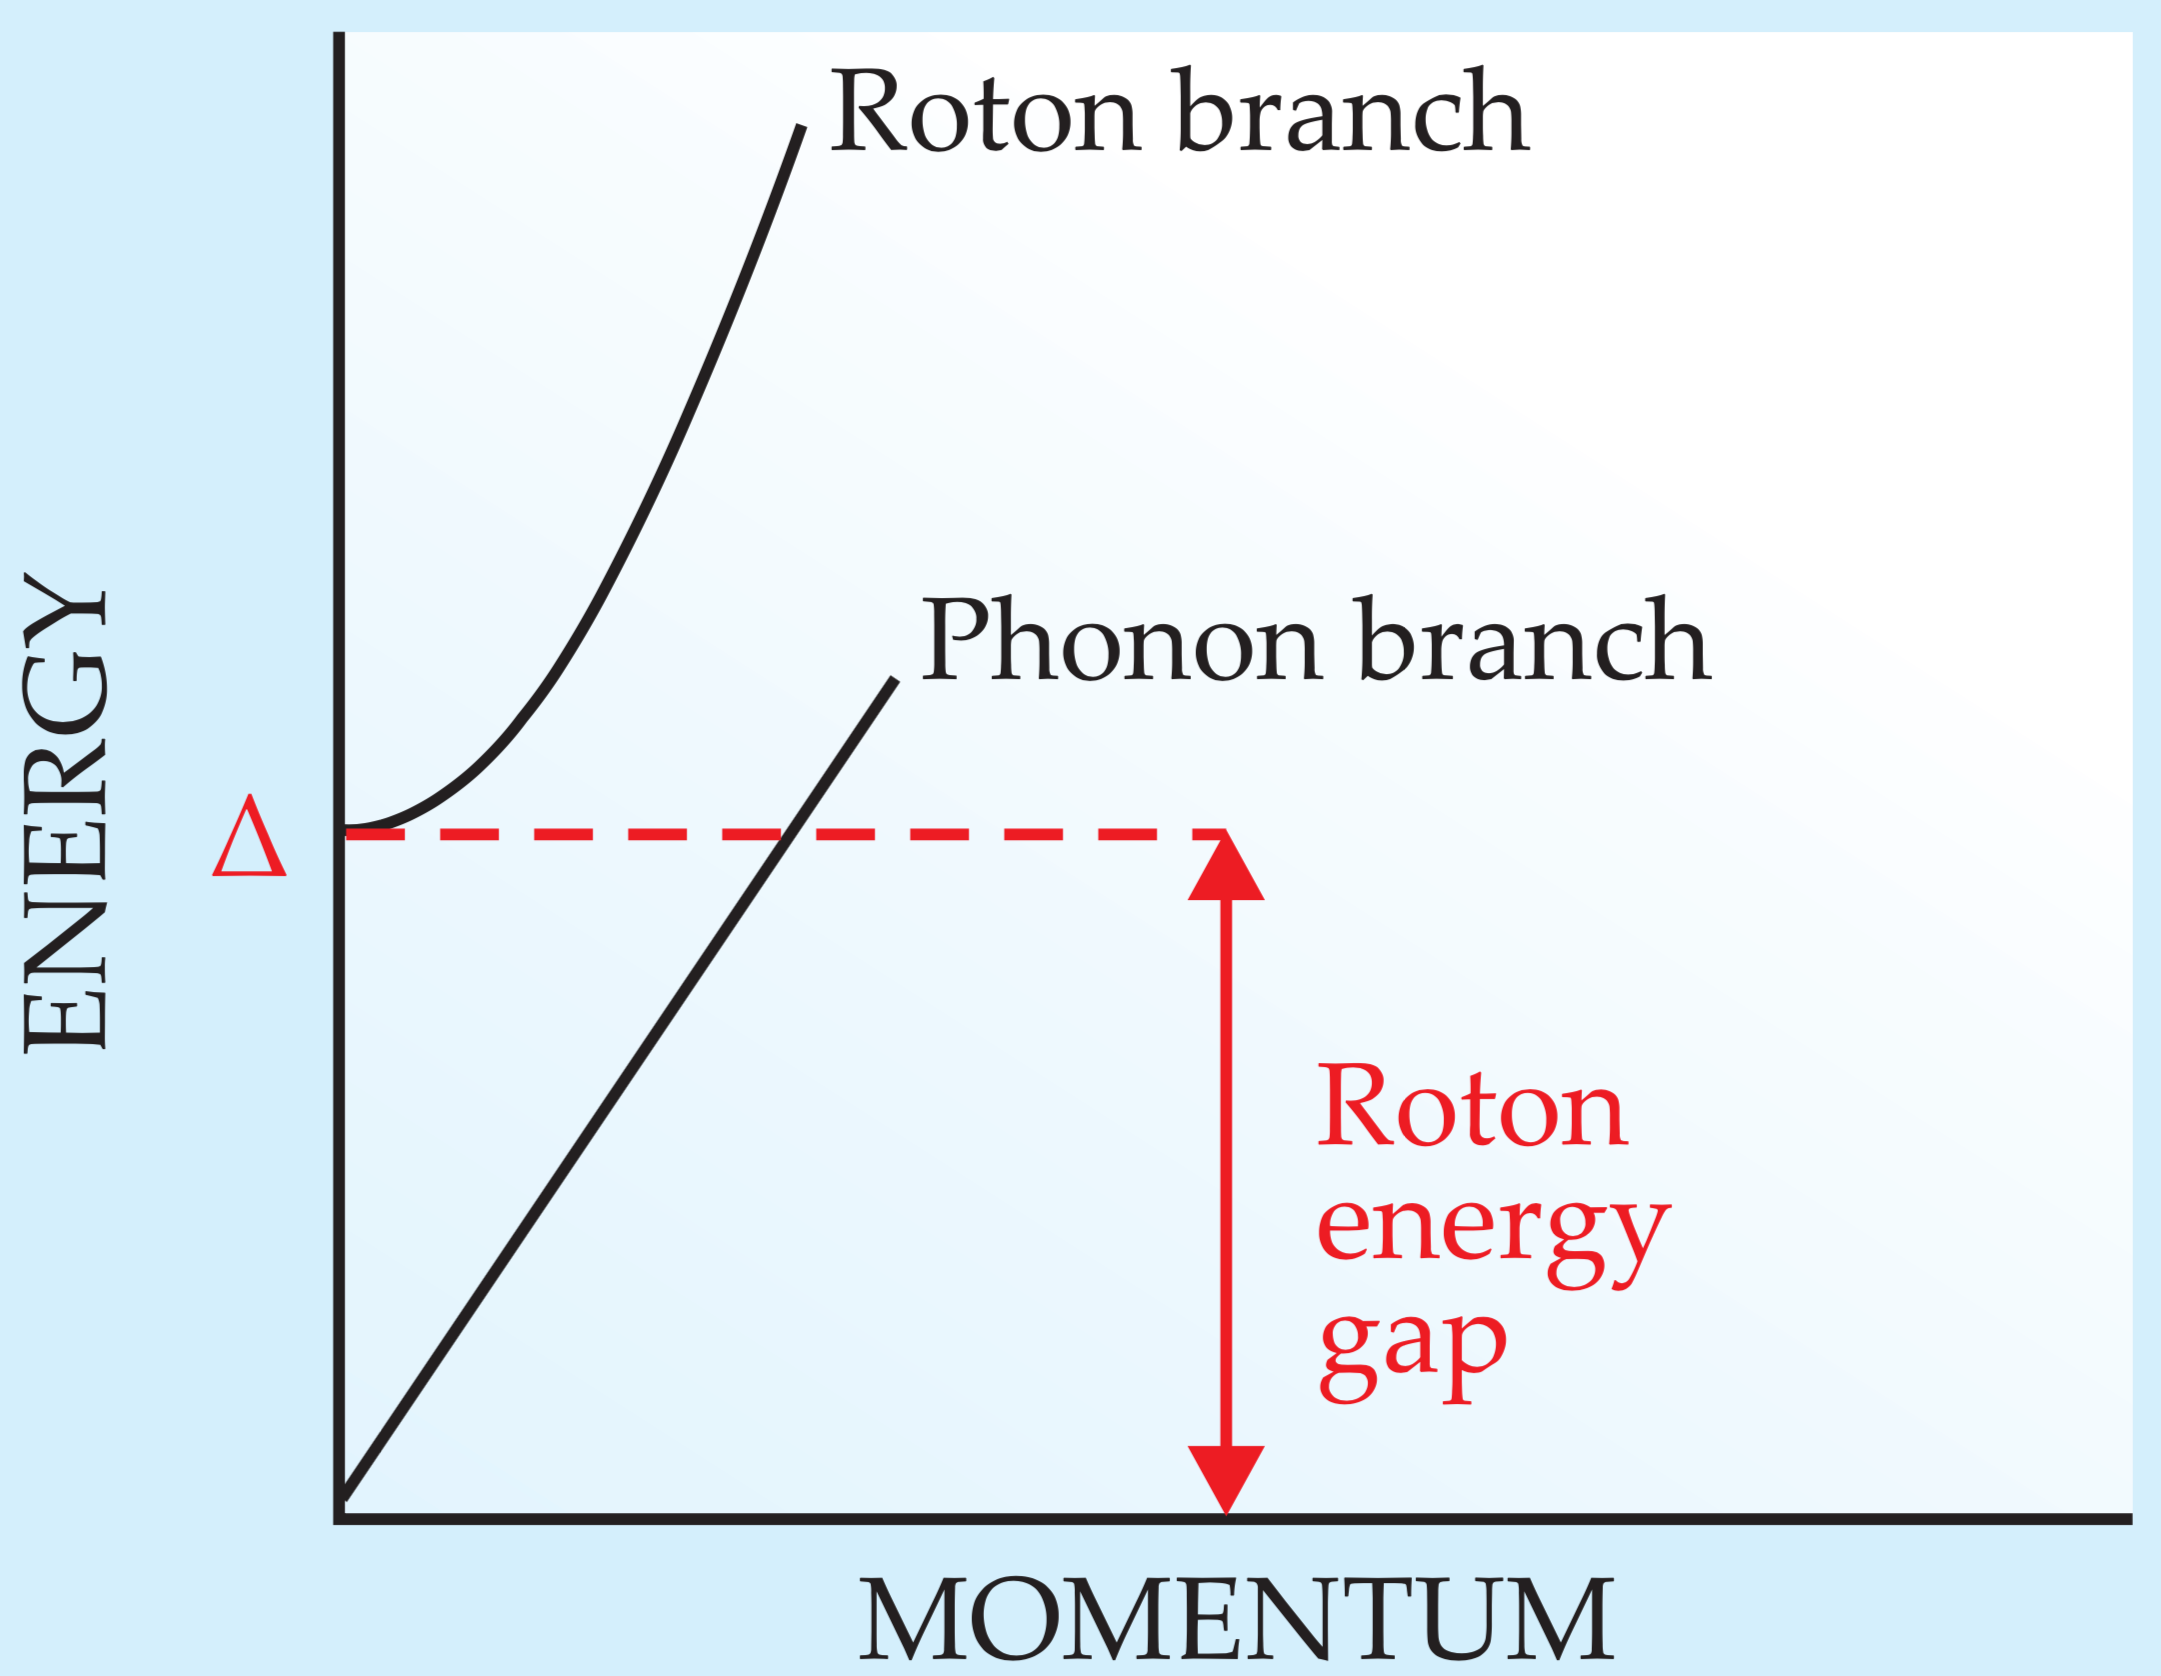
\includegraphics[width=0.45\textwidth]{phonon-roton-landau-first}
			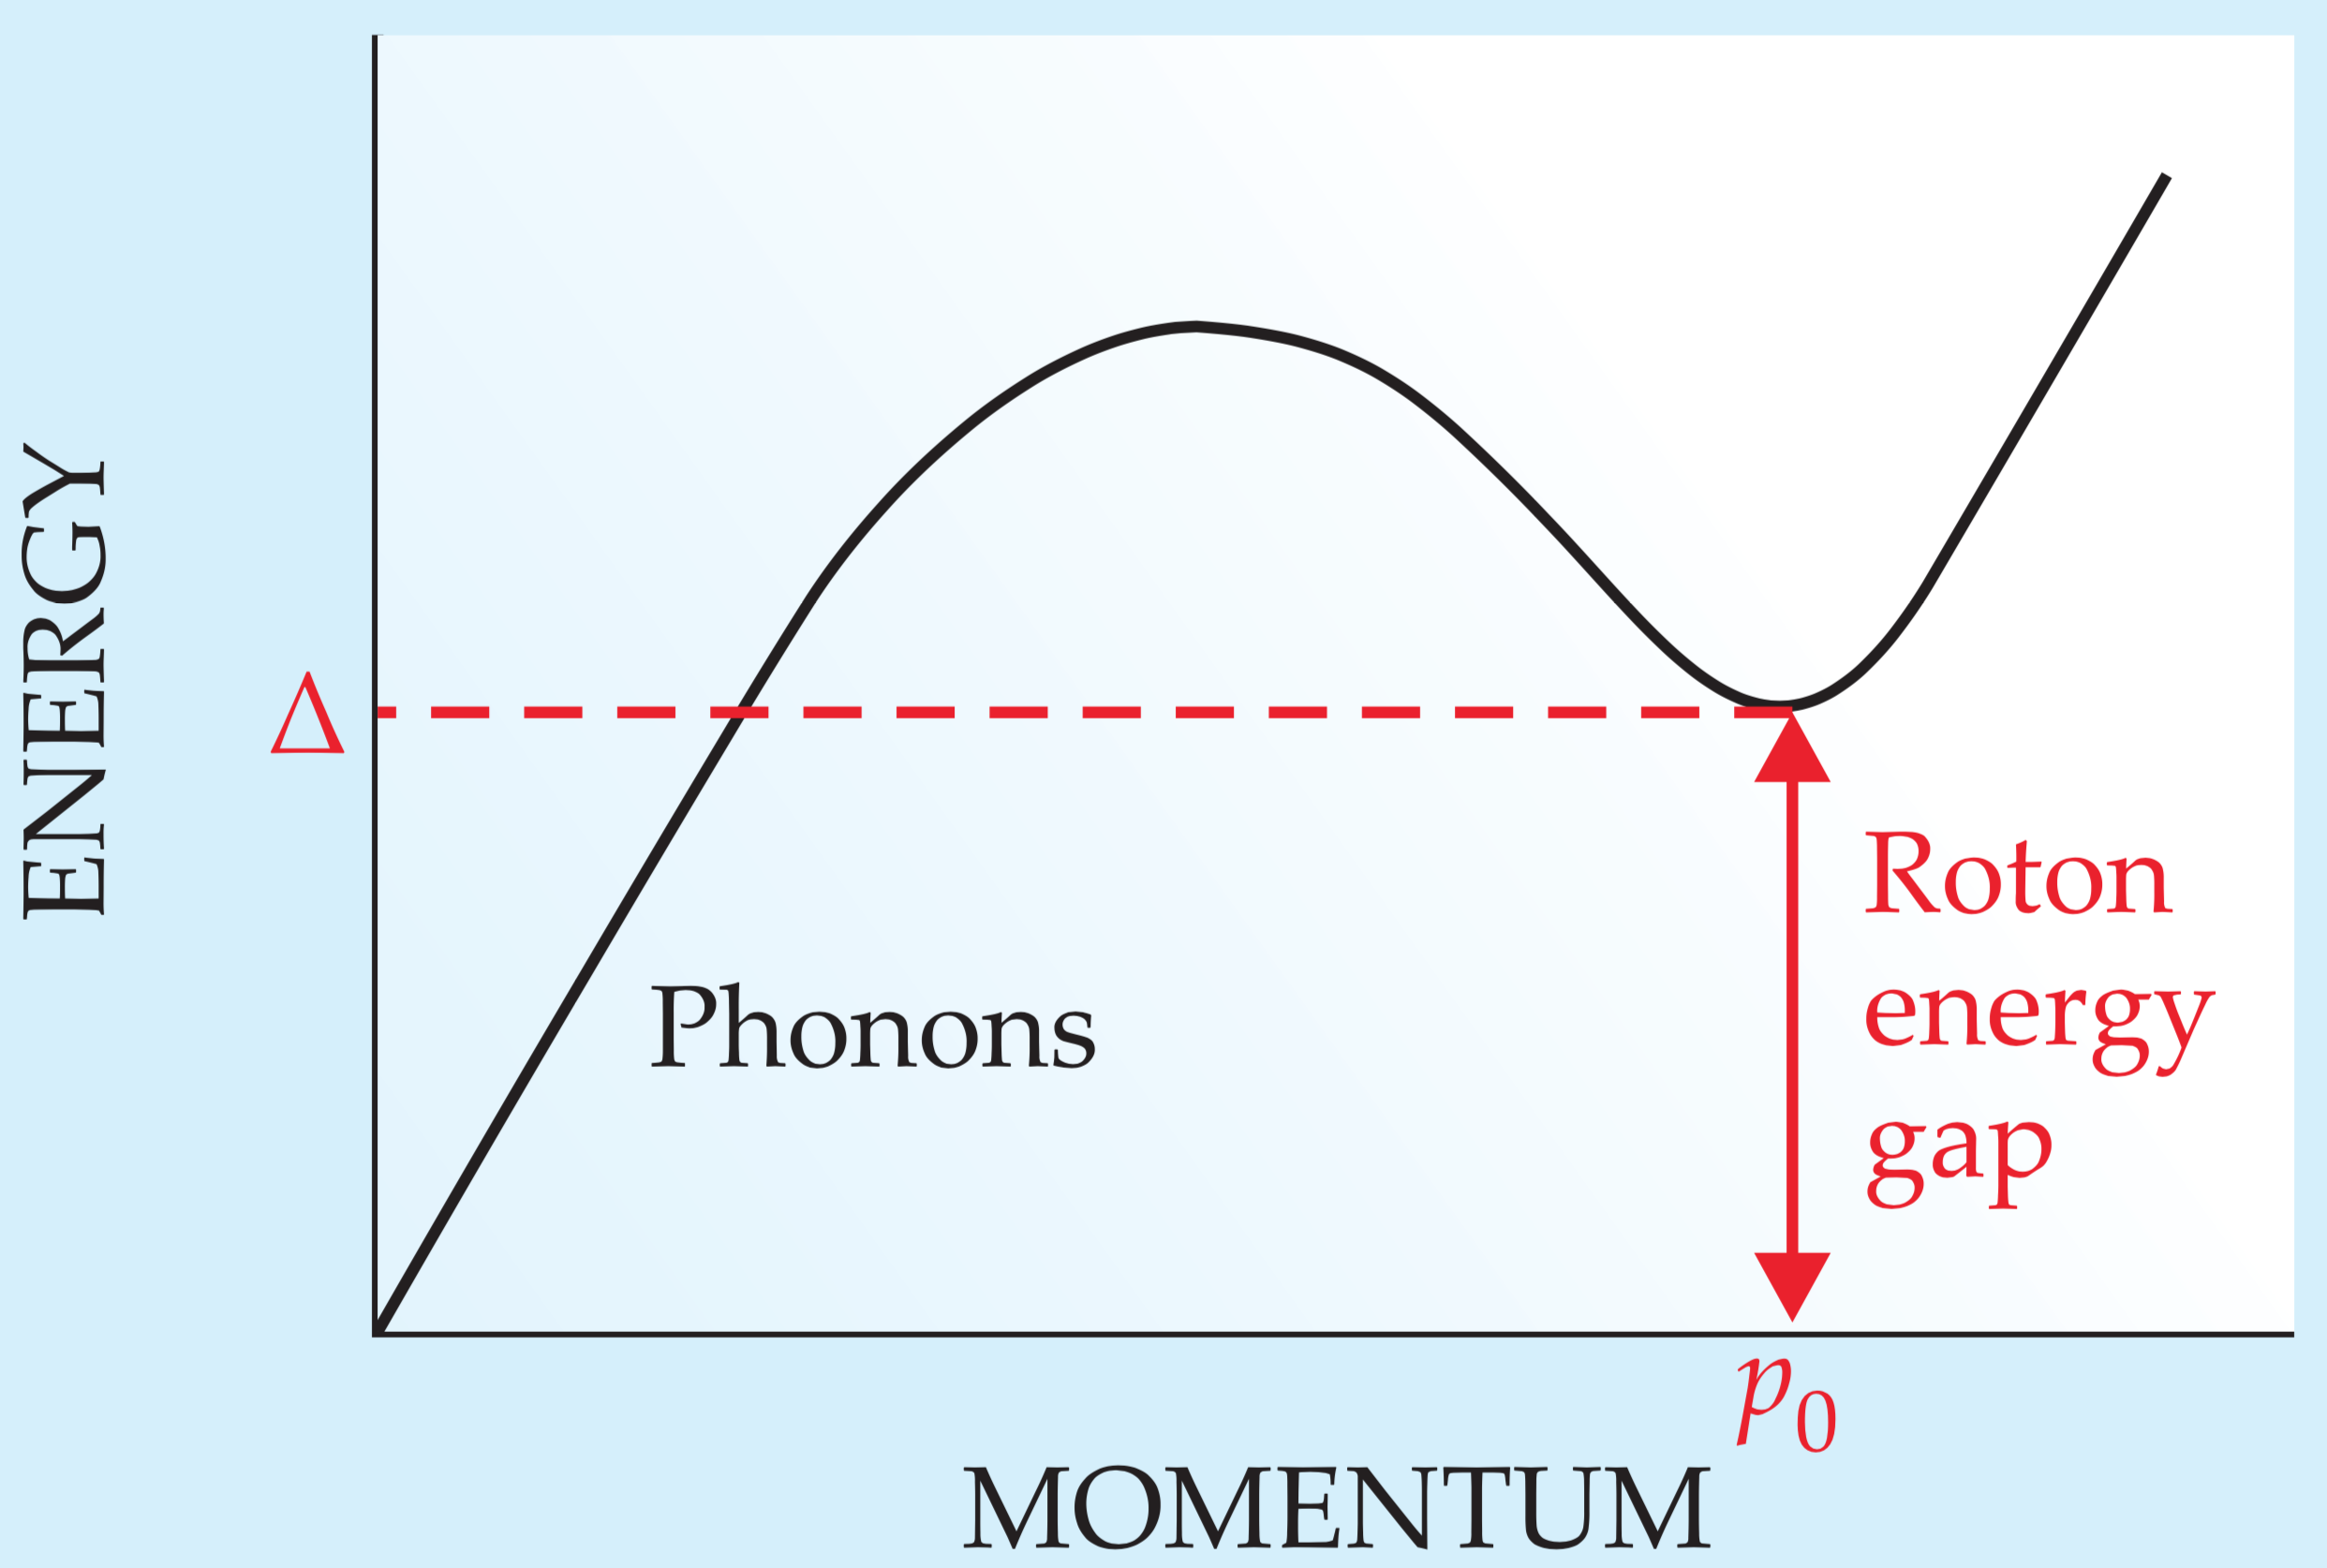
\includegraphics[width=0.45\textwidth]{phonon-roton-bogoliubov}
		\end{center}
		\caption{Left: Lev Landau's 1941 energy dispersion curve for the excitations in liquid helium below $T_\lambda$. It exhibits a phonon- and a roton branch. The slope of the linear phonon branch corresponds to the velocity of sound. Right: Lev Landau's (Bogoliubov's) 1947 corrected dispersion curve. The roton-branch is no longer a separate excitation branch but rather an extension of the phonon-branch.}
		\label{fig:phonon-roton}
	\end{figure}

	A theoretical demonstration that phonons and rotons are collective excitations of the liquid came in the form of a 1947 paper by Nikolay Bogolyubov[ref]. The intimate relationship between superfluidity and Bose-Einstein condensation was not universally accepted until 1995 when Cornell and Wienman in Colorado and Ketterle at MIT discovered BEC in rubidium quantum gases[ref].\\
	
	Until the 1980, most experimental and theoretical work was done on bulk systems, i.e. systems of the order of $N_A$ number of atoms. It was only in the last couple of decades that advancements in technology enabled experimentalists to create nanoscale sized superfluid helium droplets. From the early 1990's onwards, superfluid helium nano-droplets became an active field of study, both experimentally and theoretically. Surely, the finite size of these droplets would impose some interesting properties compared to bulk liquid helium. The helium-helium interaction is already weak in bulk liquid helium and in finite self-bound systems such as droplets is even weaker, e.g. the binding energy per atom is $<\!7.17\unit{K}$. Because of this helium droplets cool down very rapidly, reaching their limiting temperature of about $0.38\unit{K}$ in microseconds. Pure helium droplets are neutral systems and its properties like their size, binding energy and excitation spectra, are not easy to determine experimentally and are usually obtained by indirect methods. This didn't stop the theoreticians describe doped $^4$He$_N$ droplets using a wide variety of approaches depending on the size and character of the droplets ranging from Quantum Monte Carlo, Hypernetted-Chain/Euler-Lagrange, Variational Monte Carlo, [\emph{insert more methods here, before arriving at DFT}].\\
	
	Another important property of helium droplets is their ability to pickup any kind of dopants with which they collide, binding them, depending on the relative strength of the He-dopant interaction compared to the He-He interaction, either to their surface (e.g. the alkalies) or absorb them into their interior. They can therefore be doped with almost any kind of atomic or molecular species where they can form new complexes.
	
	\subsection{Bose-Einstein condensation and superfluidity}		
	Bose-Einstein Condensation
	\begin{itemize}
		\item Long-range order: diagonal density, Bogolyubov approximation, order parameter
		\item Ideal Bose-gas in a box: thermal wavelength $\lambda_T$ (3.14), critical temperature $T_c$ (3.28), condensate fraction $N_0$ (3.31), $\epsilon(p)=p^2/2m$
		\item Weakly-interacting Bose gas: Bogolyubov's famous dispersion law $\epsilon(\vec{p})=\qty[\frac{gn}{m}p^2+\qty(\frac{p^2}{2m})^2]^{1/2}$. Small $p$, $\epsilon(p)=cp$, phonons.
		\item Non-uniform Bose-gases at T=0: Gross-Pitaevskii, irrotational velocity flow, vortex lines, rings and solitons
		\item remind order parameter
		\item explain difference between wave function and order parameter.
	\end{itemize}

	\section{BEC}
		Condensate fraction
		\begin{align}
			\frac{N_0}{N} = 1-\qty(\frac{T}{T_0})^{3/2},
		\end{align}
		where
		\begin{align}
			T_0(\rho) = \frac{\hbar^2}{2mk_\mathrm{B}}\qty(\frac{4\pi^2\rho}{2.315(2s+1)})^{2/3},\label{eq:T0}
		\end{align}
		the critical temperature and $s$ the spin number. For $^4$He with a bulk saturation density of $\rho=2.22\,\mathrm\AA^{-3}$, $T_0\approx 2.35\,\mathrm{K}$. The condition $T<T_0$ for BEC occurrence, using Eq. (\ref{eq:T0}), can be cast the form
		\begin{align}
			\rho\lambda_{\mathrm{Th}}^3>14.546(2s+1),
		\end{align}
		where $\lambda_{\mathrm{Th}} \vcentcolon= h/\sqrt{2mk_\mathrm{B}T}$ the \emph{thermal de Broglie wavelength}. For $^4$He at $T=0.4\,\mathrm{K}$, $\lambda_{\mathrm{Th}}\approx 24.5$\,\AA. Comparing this to superfluid $^4$He's mean inter-particle distance $\langle r_4 \rangle \sim \qty(V/N)^{1/3}=2.22\sqrt[3]{4\pi/3}\approx 3.58$\,\AA, we see that $\lambda_{\mathrm{Th}}\approx 7\times\langle r_4 \rangle $; the system is very quantum-like.
	
	\subsection{Long-range order}
		On	e-body density matrix:
		\begin{align}
			n^{(1)}(\vec{r},\vec{r}') \vcentcolon=\expval{\hat{\Psi}^\dagger(\vec{r})\hat{\Psi}(\vec{r}')}
		\end{align}
		Diagonal density:
		\begin{align}
			n(\vec{r})\vcentcolon  = n^{(1)}(\vec{r},\vec{r})
		\end{align}
		Momentum distribution
		\begin{align}
			n(\vec{p}) = \expval{\hat{\Psi}^\dagger(\vec{p})\hat{\Psi}(\vec{p})} = \frac{1}{(2\pi\hbar)^3}\int \! n^{(1)}\qty(\vec{R}+\frac{\vec{s}}{2},\vec{R}-\frac{\vec{s}}{2})\exp(-i\vec{p}\cdot\vec{s}/\hbar)\,\mathrm{d}\vec{R}\mathrm{d}\vec{s},
		\end{align}
		where $\vec{R}\vcentcolon=(\vec{r}+\vec{r}')/2$ and $\vec{s}\vcentcolon=\vec{r}-\vec{r}'$.
	
	\subsection{Bogolubov ansatz}
	\begin{align}
		\hat{\Psi}(\vec{r})=\Psi_0(\vec{r})+\delta\hat{\Psi}(\vec{r}),
	\end{align}
	where $\hat{\Psi}(\vec{r})=\sum_{i\neq 0}\varphi_i\hat{a}_i$ and $\Psi_0(\vec{r})=\sqrt{N_0}\varphi_0$ is called the ``wave function of the condensate''. It is a complex quantity characterised by a real-valued modulus $\Phi$ and phase $S$:
	\begin{align}
		\Psi_0(\vec{r}) = \Phi(\vec{r})\mathrm{e}^{iS(\vec{r})}
	\end{align}
	
	\section{Superfluidity}
		\subsection{Landau's criterion}
			\begin{align}
				v<v_c = \min_{\vec{p}}\frac{\epsilon(\vec{p})}{p}
			\end{align}
			
			For an ideal Bose gas $\epsilon(\vec{p})=p^2/2m$, so 
			\begin{align}
				v_c &= \min_{\vec{p}}\frac{\epsilon(\vec{p})}{p} \\
					&= \min_{\vec{p}}\frac{p}{2m} \\
					&= 0
			\end{align}
			It is not a superfluid. But for a weakly interacting Bose gas, $\epsilon(\vec{p})=\sqrt{\frac{gn}{m}p^2+\qty(\frac{p^2}{2m})^2}$ (Bogoliubov's dispersion law for elementary excitations, 1947), so
			\begin{align}
				v_c &=\min_{\vec{p}}\sqrt{\frac{gn}{m}+\frac{p^2}{4m^2}} \\
					&= \sqrt{\frac{gn}{m}} \\
					&= c,
			\end{align}
			the speed of sound. Here $g=\frac{4\pi\hbar^2a}{m}$, and $a$ the $s$-wave scattering length. The weakly interacting Bose gas is a superfluid.	
			
		\subsection{Rotation in superfluids}
			\begin{itemize}
				\item super fluid flow is irrotational
				\item Angular momentum and vorticity are quantised.
			\end{itemize}
			
	\subsection{State of the art}
		* What has been done in the last two decades
			- Manuel's review paper from 2006
			- Manuel's review paper from 2017
		* droplets as and ideal medium for chemistry
			- characterisation of the photo-excitation dynamics of Alkalis
		* droplets as a medium to study atomic cluster formation and dynamics
	
	\subsection{Structure of the thesis}
		\subsubsection{Part I}
			This part of the thesis will study the real-time dynamics of a single electronically excited Rubidium (Rb) atom, residing in the surface dimple of a helium nano-droplet, excited from the ground state 5s$^2\Sigma_{1/2}$ to the 5p$^2\{\Sigma,\Pi\}$ and 6p$^2\{\Sigma,\Pi\}$ manifold. This will be a mixed experimental and theoretical study. The results will be presented in two published articles:
			
			\emph{Imaging Excited-State Dynamics of Doped He Nanodroplets in Real-Time} will focus on imaging and characterising the dynamics using femtosecond spectroscopy and  time-dependent density functional theory.
			
			\emph{Desorption dynamics of RbHe-exciplexes off He nanodroplets induced by spin relaxation} is a combined experimental and theoretical investigation of the formation of free RbHe-exciplex molecules from laser-excited Rb-doped He nanodroplets through the mechanism of electronic spin relaxation. The role of relaxation of internal degrees of freedom of the RbHe exciplex in the desorption process has not been explicitly addressed.

		\subsubsection{Part II}
			The second part will contain only theoretical investigations.
			- Head-on collisions between Xenon and droplets
			- Capture process of xenon and argon by quantised vortices in droplets
			










































%		Introduce superfluids and their properties
%		* Frictionless capillary flow (no viscosity)
%		* Creeping up the walls seemingly defying gravity
%		* capillary fountain
%		* second sound: heat propagating in waves with a constant speed of "second sound" instead of diffusion
%		* Fluid is irrotational
%		* Vorticity is quantised
	 

%%		E, 1908, July 10:		Kamerlingh Onnes, Liquefaction of helium-4,\\
%%		E, 1932, July:			John C. McLennan, Observed liquid helium stops boiling
%below 2.2 K. \\
%%		E, 1932:				W.H. Keesom, A.P. Keesom, observed a singularity in the specific
%heat at T=2.2 K and called it the lambda-temperature, because of the shape of
%the temperature dependence of the specific heat resembling the greek letter
%lambda.\\
%%		E, 1935, February 16:	E.F. Burton, measured sharply decreasing viscosity
%below 2.2 K\\
%%		T, 1935, August 16:		F. London, found that the magnitude of the zero-point
%energy of helium-4 is comparable to the Van der Waals interaction. This
%explains why helium doesn't freeze at T=0 at normal atmospheric pressure.\\
%%		E, 1936, May:			W.H. Keesom, A.P. Keesom, Observed abnormally thermal
%conductance, calling it 'supra-heat-conducting'\\
%%		E, 1937, July 10:		J.F. Allen,R. Peierls, M. Zaki Uddin, also observed
%abnormally high heat conductance. This was the reason for the liquid not
%boiling below 2.2 K\\
%%		E, 1937, December 3:	Kapitza, observed that below lambda-point viscosity of
%helium II is roughly 1500 smaller than helium I at normal pressure. In analogy
%with superconductors he concluded that helium below lambda enters a special
%state which he called superfluid.	This was the first mention of the word
%superfluid.\\
%%		E, 1937, December 22:	Allen and Misener (1938) discovered that helium-ii is
%not just a liquid with a very low viscosity, but that its hydrodynamics
%required a completely new interpretation.\\
%%		E, 1938, 05 February: 	J.F. Allen, discovery of fountain effect\\
%%		T, 1938, April 9:		F. London, connects behaviour of helium-II to BEC (ideal
%BE-gas). calculated Tc=3.09 K and Cv(t) for ideal BE-gas and they were very
%close to helium-II. He concluded that it was difficult not to imagine a
%connection to BEC\\
%%		T, 1938, May 21:		L. Tisza, birth of the 2-fluid model\\
%
%					which leads to 
%
%	Explanation of superfluidity by 
%		* Fritz London (April 1938, London, F., Nature, 141, 643 (1938))
%l-transition in liquid helium is analogous to Bose-Einstein condensation
%%		* Laszlo Tisza (May 1938, L. Tisza, Nature, 141, 913 (1938)) extended
%London's proposal by invoking a two-fluid model for helium II, which could
%qualitatively explain the observed transport phenomena, including the fountain
%effect.
%%		* Lev Landau (1941) if the spectrum of elementary excitations satisfies
%suitable criteria, the flow of of the fluid cannot dissipate energy. Postulated
%"phonons" and "rotons" and the famous Landau criterion for superfluidity
%%		* Nikolay Nikolayevich Bogolyubov (Oct. 12, 1946. Publ. 1947): Derivation of
%the elementary excitation spectrum from a molecular theory, making no
%assumptions about the structure of the energy spectrum.


%	\section{Random stuff about BEC}
%	Most general (time-independent) many-body Hamiltonian
%	\begin{align}
%		H(\vec{r}_1,\ldots,\vec{r}_N, \vec{p}_1,\ldots,\vec{p}_N) =
%\sum_{i=1}^N
%\qty(-\frac{\hbar^2}{2m_i}\nabla_{\vec{r}_i}^2)+V(\vec{r}_i,\ldots,\vec{r}_N)
%	\end{align}
%	And accompanying Schrödinger equation to solve
%	\begin{align}
%		i\hbar\frac{\partial}{\partial t}\Psi(\vec{r}_1,\ldots,\vec{r}_N,t) =
%\qty[\sum_{i=1}^N
%\qty(-\frac{\hbar^2}{2m_i}\nabla_{\vec{r}_i}^2)+V(\vec{r}_i,\ldots,\vec{r}_N)
%]\Psi(\vec{r}_1,\ldots,\vec{r}_N,t)
%	\end{align}
%For a 2-body system and a potential that only depends on the relative
%coordinate $\vec{r}_1-\vec{r}_2$ the Hamiltonian reduces reduces to
%	\begin{align}
%		H(\vec{r}_1,\vec{r}_2) =
%-\qty(\frac{\hbar^2}{2m_1}\nabla_{\vec{r}_1}^2+\frac{\hbar^2}{2m_2}\nabla_{\vec
%{r}_2}^2)+V(\vec{r}_1-\vec{r}_2)
%	\end{align}
%By either introducing the relative coordinate $\vec{r}$ and the center-of-mass
%(CM) coordinate $\vec{R}$, or the relative momentum
%$\vec{p}$ and the total momentum $\vec{P}$, we can consider the motion of the
%CM itself ($\vec{R}$) and the motion relative to the CM
%	($\vec{r}$):
%	\begin{align}
%		H(\vec{R},\vec{r}) =
%-\qty(\frac{\hbar^2}{2M}\nabla_{\vec{R}}^2+\frac{\hbar^2}{2\mu}\nabla_{\vec{r}}
%^2)+V(\vec{r}),
%	\end{align}
%with $M=m_1+m_2$ and $\mu=\frac{m_1m_2}{m_1+m_2}$ (reduced mass of the system).
%	Schrödinger equation to solve
%	\begin{align}
%i\hbar\frac{\partial}{\partial t}\Psi(\vec{R},\vec{r},t) &=
%H(\vec{R},\vec{r})\Psi(\vec{R},\vec{r},t) \\
%&=
%\qty[-\qty(\frac{\hbar^2}{2M}\nabla_{\vec{R}}^2+\frac{\hbar^2}{2\mu}\nabla_
%{\vec{r}}^2)+V(\vec{r})]
%		\Psi(\vec{R},\vec{r},t) \label{eq:2b-se}
%	\end{align}
%	Assuming a separable solution and the given time-independence of the potential
%	\begin{align}
%\Psi(\vec{R},\vec{r},t) =
%\Phi(\vec{R})\psi(\vec{r})\mathrm{e}^{-i(E_{CM}+E)t/\hbar}
%	\end{align}
%and the 2-body Schrödinger equation (\ref{eq:2b-se}) separates into two
%mutually time-independent ODEs
%	\begin{align}
%-\frac{\hbar^2}{2M}\nabla_{\vec{R}}^2\Phi(\vec{R}) &= E_{CM}\Phi(\vec{R})
%\label{eq:se-fp}\\
%\qty[-\frac{\hbar^2}{2\mu}\nabla_{\vec{r}}^2 + V(\vec{r})]\psi(\vec{r}) &=
%E\psi(\vec{r}). \label{eq:se-muv}
%	\end{align}
%ODE (\ref{eq:se-fp}) describes the center of mass motion for a free particle
%with mass $M$ and energy
%$E_{CM}$. In one dimension the time-\emph{dependent normalizable} solution for
%such a particle,
%initially localized between $-a$ and $a$ is an integral over plane waves over
%all frequencies
%	\begin{align}
%\Phi(X,t) =
%\frac{1}{\pi}\sqrt{\frac{a}{2}}\int_{-\infty}^{+\infty}\!\mathrm{sinc}(ka)\,
%		\exp[i\qty(kX-\frac{\hbar k^2}{2M}t)]\,\mathrm{d}k.
%	\end{align}
%ODE (\ref{eq:se-muv}) describes the motion relative to the CM of a particle of
%reduced mass $\mu$ in a potential $V(\vec{r})$.
%	For hydrogen this is the Coulomb potential. Explicitly
%	\begin{align}
%\qty[-\frac{\hbar^2}{2\mu}\nabla_{\vec{r}}^2 -
%\frac{e^2}{(4\pi\varepsilon_0)r}]\psi(\vec{r}) &= E\psi(\vec{r}),
%	\end{align}
%where it is customary to switch to spherical polar coordinates and separate the
%solutions again
%	\begin{align}
%\psi(\vec{r}) \rightarrow \psi_{E,l,m}(r,\theta,\phi) =
%R_{E,l}(r)Y_{ml}(\theta,\phi),
%	\end{align}
%where $R_{E,l}$ is the radial wave function, fully determined by the energy $E$
%and the orbital angular momentum quantum
%number $l$ and $Y_{ml}$ are the spherical harmonics, fully determined by $l$
%and the magnetic quantum number $m$.
%	
%	\section{Helium-4, a 3-body system with 2 electrons}
%The unperturbed (omit electron-electron repulsion) ground state (as obtained by
%the `single particle model')
%	\begin{align}
%\psi_0^{(0)}(r_1,r_2) &= \psi_{1\mathrm{s}(r_1)}\psi_{1\mathrm{s}(r_2)} \otimes
%		\frac{1}{\sqrt{2}}\qty(\ket{\uparrow\downarrow}-\ket{\downarrow\uparrow}) \\ 
%&= \frac{8}{\pi}\exp[-2(r_1+r_2)] \otimes
%\frac{1}{\sqrt{2}}\qty(\ket{\uparrow\downarrow}-\ket{\downarrow\uparrow})
%	\end{align}
%Or in the `central field approximation' with effective nuclear charge
%$Z_e=1.70$
%	\begin{align}
%\psi_0(r_1,r_2) =
%\frac{4.913}{\pi}\exp[-1.70(r_1+r_2)]\otimes\frac{1}{\sqrt{2}}\qty(\ket
%{\uparrow\downarrow}-\ket{\downarrow\uparrow})
%	\end{align}

\end{document}